\chapter[Знакомство с языком \Sys{С++}]{Знакомство с языком \Sys{С++}}

В этой главе читатель напишет свои первые программы на языке \Sys{С(\Sys{С++})}, 
познакомится с основными этапами перевода программы
с языка \Sys{C++} в машинный код. Второй параграф главы посвящён 
знакомству со средой \Sys{Qt Creator}.

\section[Первая программа на \Sys{C++}]{Первая программа на \Sys{C++}}
Знакомство с языком \Sys{С++} начнём с написания программ, предназначенных 
для решения нескольких несложных задач.

\prg{Заданы две стороны прямоугольника a, b. Найти его площадь и
периметр.}{gl1:prg1}

Как известно, периметр прямоугольника $P=2\cdot(a+b)$, а его площадь 
%вычисляется по формуле 
$S=a\cdot{b}$. 
Ниже приведён текст программы. 

\begin{lstlisting}[numbers=left, numberstyle=\tiny, stepnumber=1, numbersep=5pt]
#include <iostream> 
using namespace std; 
int main() 
{ 
    float a,b,s,p; 
    cout<<"a="; 
    cin>>a; 
    cout<<"b="; 
    cin>>b; 
    p=2*(a+b); 
    s=a*b; 
    cout << "`Периметр прямоугольника равен` " << p <<endl; 
    cout << "`Площадь прямоугольника равна` " << s <<endl; 
    return 0; 
}
\end{lstlisting}

Давайте построчно рассмотрим текст программы и познакомимся 
со структурой программы на \Sys{С++} и с некоторыми операторами
языка. 

\Emph{Строка 1.} Указывает компилятору (а точнее, препроцессору), что надо использовать функции из стандартной
библиотеки \index{Библиотека!iostream}\Sys{iostream}. Библиотека \Sys{iostream} нужна для организации ввода с
помощью инструкции \Sys{cin} и вывода --- с помощью \Sys{cout}. В программе на языке \Sys{C++} должны
быть подключены все используемые библиотеки.

\Emph{Строка 2.} Эта строка обозначает, что при вводе и выводе с помощью \Sys{cin} и
\Sys{cout} будут использоваться стандартные устройства (клавиатура и экран), если эту строку не указывать,
то каждый раз при вводе вместо \Sys{cin} надо будет писать \Sys{std::cin}, а вместо
\Sys{cout --- std::cout}.

\Emph{Строка 3.} Заголовок главной функции (главная функция имеет имя \Sys{main}). В простых программах
присутствует только функция \Sys{main()}.

\Emph{Строка 4.} Любая функция начинается с символа \Sys{\{}.

\Emph{Строка 5.} Описание вещественных (\Sys{float}) переменных \Sys{a} (длина одной стороны
прямоугольника), \Sys{b} (длина второй стороны прямоугольника), \Sys{s} (площадь
прямоугольника), \Sys{p} (периметр прямоугольника). Имя переменной\footnote{В 
литературе равнозначно используются термины «имя переменной» и
«идентификатор».} состоит из латинских букв, цифр и символа подчёркивания. Имя не может начинаться
с цифры. В языке \Sys{С++} большие и малые буквы различимы. Например, имена \Sys{PR\_1},
\Sys{pr\_1}, \Sys{Pr\_1} и \Sys{pR\_1} --- разные.

\Emph{Строка 6.} Вывод строки символов \Sys{a=} с помощью \Sys{cout}. Программа выведет
подсказку пользователю, что необходимо вводить переменную \Sys{a}

\Emph{Строка 7.} Ввод вещественного числа \Sys{a} с помощью \Sys{cin}. В это момент
программа останавливается и ждёт, пока пользователь введёт значение переменой \Sys{a} с клавиатуры.

\Emph{Строка 8}. Вывод строки символов \Sys{b=} с помощью \Sys{cout}.

\Emph{Строка 9.} Ввод вещественного числа \Sys{b} с помощью \Sys{cin}.

\Emph{Строка 10.} Оператор присваивания для вычисления периметра прямоугольника (переменная \Sys{p}) по
формуле  $2\cdot(a+b)$ . В операторе присваивания могут использоваться круглые скобки и знаки операций: + (сложение),
- (вычитание), * (умножение), / (деление).

\Emph{Строка 11.} Оператор присваивания для вычисления площади прямоугольника.

\Emph{Строка 12.} Вывод строки «\Sys{Периметр прямоугольника равен }» и значения \Sys{p} на экран. Константа
\Sys{endl} хранит строку <<\textbackslash{n}>>, которая предназначена для
перевода курсора в новую строку дисплея\footnote{Обращаем внимание читателя, что символ пробел является обычным
символом, который ничем не отличается от остальных. Для вывода пробела на экран его надо явно указывать в строке
вывода.}. Таким образом строка 

\Sys{cout} {\textless}{\textless} \Sys{"Периметр прямоугольника равен " {\textless}{\textless} p
{\textless}{\textless}endl;} 

выводит на экран текст \Sys{"Периметр прямоугольника равен "}\footnote{С пробелом после слова
«равен».}, значение переменной \Sys{p}, и переводит курсор в новую строку.

\Emph{Строка 13.} Вывод строки \Sys{"Площадь прямоугольника равна "}, значения площади
прямоугольника \Sys{s}, после чего курсор переводится в новую строку дисплея.

\Emph{Строка 14.} Оператор \Sys{return}, который возвращает значение в
операционную систему. Об этом подробный разговор предстоит в п.~\ref{ch04:9} %4.9. 
Сейчас следует запомнить, если программа
начинается со строки \Sys{int main()}, последним оператором должен быть
\Sys{return 0}\footnote{Вообще говоря, вместо нуля может быть любое целое число.}.

\Emph{Строка 15.} Любая функция (в том числе и \Sys{main}) заканчивается символом \}.

Мы рассмотрели простейшую программу на языке \Sys{С++}, состоящую из операторов ввода 
данных, операторов присваивания (в
которых происходит расчет по формулам) и операторов вывода. 

Любая программа на языке \Sys{С++} представляет собой одну или несколько функций. 
В любой программе \Emph{обязательно}
должна быть одна функция \index{Функция!main}\Sys{main()}. C этой функции начинается 
выполнение программы. Правилом хорошего
тона в программировании является разбиение задачи на подзадачи, и в главной функции 
чаще всего должны быть операторы
вызова других функций. Общую структуру любой \index{Структура программы}программы на 
языке \Sys{C++} можно записать следующим
образом. 

\begin{lstlisting}
`Директивы препроцессора`
`Объявление глобальных переменных`
`Тип\_результата` f1(`Список\_переменных`)
{
`Операторы`
}
`Тип\_результата` f2(`Список\_переменных`)
{
`Операторы`
}

...

`Тип\_результата` fn(`Список\_переменных`)
{
`Операторы`
}
`Тип\_ результата` main(`Список\_переменных`)
{
`Операторы`
}
\end{lstlisting}

На первом этапе знакомства с языком мы будем писать программы, состоящие только из функции main, без использования
глобальных переменных. Структура самой  простой на С(\Sys{С++}) имеет вид.
\begin{lstlisting}
`Директивы препроцессора`
`Тип\_ результата` main(`Список\_переменных`)
{
`Операторы`
}
\end{lstlisting}
Введенная в компьютер программа на языке \Sys{С++} должна быть переведена в двоичный машинный код (должен быть сформирован
исполняемый файл). Для этого существуют специальные программы, называемые трансляторами. Все
\index{Транслятор}трансляторы  делятся на два класса:

\begin{itemize}
\item \index{Интерпретатор}\emph{интерпретаторы} --- трансляторы, которые переводят 
каждый оператор программы в машинный код, и по мере перевода операторы
выполняются процессором; 
\item \index{Компилятор}\emph{компиляторы} переводят всю программу целиком, и если 
перевод всей программы прошел без ошибок, то полученный двоичный код можно
запускать на выполнение. 
\end{itemize}
Процесс перевода программы в машинный код называется \emph{трансляцией}. 
Если в качестве транслятора выступает компилятор, то используют термин \emph{компиляция}%
~программы. При переводе программы с языка \Sys{С++} в машинный код используются именно 
компиляторы, и поэтому применительно к
языку \Sys{С++} термины «компилятор» и «транслятор» эквивалентны.

Рассмотрим основные этапы обработки компилятором программы на языке \Sys{С++} и формирования машинного кода.

\begin{enumerate}
\item Сначала программа обрабатывается препроцессором\footnote{Препроцессор --- это программа, которая преобразовывает
текст директив препроцессора в форму, понятную компилятору. О данных на выходе препроцессора говорят, что они находятся
в препроцессированной форме.}, который обрабатывает директивы препроцессора, в нашем случае это директивы включения
заголовочных файлов (файлов с расширением \Emph{.h}) --- текстовых файлов, в которых содержится описание используемых
библиотек. В результате формируется полный текст программы, который поступает на вход компилятора. 
\item Компилятор разбирает текст программ на составляющие элементы, проверяет синтаксические ошибки и в случае их
отсутствия формирует объектный код (файл с расширением \Emph{.o} или .\Emph{obj}). Получаемый на этом этапе
двоичный код не включает в себя двоичные коды библиотечных функций и функций пользователя.
\item \emph{Компоновщик} подключает к объектному коду программы объектные модули библиотек и других 
файлов (если программа состоит из нескольких
файлов) и генерирует исполняемый код программы (двоичный файл), который уже можно запускать на выполнение. Этот этап
называется компоновкой или сборкой программы.
\end{enumerate}
После написания программы ее необходимо ввести в компьютер. В той книге будет рассматриваться работа на языке \Sys{C++} в
среде \Sys{Qt Creator}\footnote{Тексты программ, приведённые в первой части книги (главы 1--9), без серьёзных изменений
могут быть откомпилированы с помощью любого современного компилятора с языка \Sys{С}(\Sys{С++}). Авторы протестировали все
программы из первой части книги с помощью  \Sys{QT Creator} и  \Sys{IDE Geany} (с использованием g++ версии~4.8).}. 
Поэтому перед
вводом программы в компьютер надо познакомиться со средой программирования.

\section[Среда программирования \Sys{Qt Creator}]{Среда программирования \Sys{Qt Creator}}
\index{Среда~программирования \Sys{Qt~Creator}}Среда программирования \Sys{Qt Creator} 
(IDE \Sys{IDE QT Creator}) находится в репозитории
большинства современных дистрибутивов Linux (OC Linux Debian, OC Linux Ubuntu, OC ROSA Linux, ALT Linux и др.).
Установка осуществляется штатными средствами вашей операционной системы (менеджер пакетов Synaptic и др.) из
репозитория, достаточно установить пакет qtcreator, необходимые пакеты и библиотеки будут доставлены  автоматически.
Последнюю версию IDE \Sys{Qt Creator} можно скачать на сайте QtProject (\url{http://qt-project.org/downloads}). Скачанный
установочный файл имеет расширениe \Emph{.run}. Для установки приложения, необходимо запустить его на выполнение.
Установка проходит в графическом режиме. После запуска программы пользователь увидит на экране окно, подобное
представленному на рис. \ref{ch01:refDrawing0}\footnote{Окно на вашем компьютере визуально может несколько отличаться от
представленного на рис. \ref{ch01:refDrawing0}, авторы использовали IDE \Sys{Qt Creator} версии~2.6.2, основанную на QT~5.0.1.}.


\begin{figure}[htb]
\begin{center}
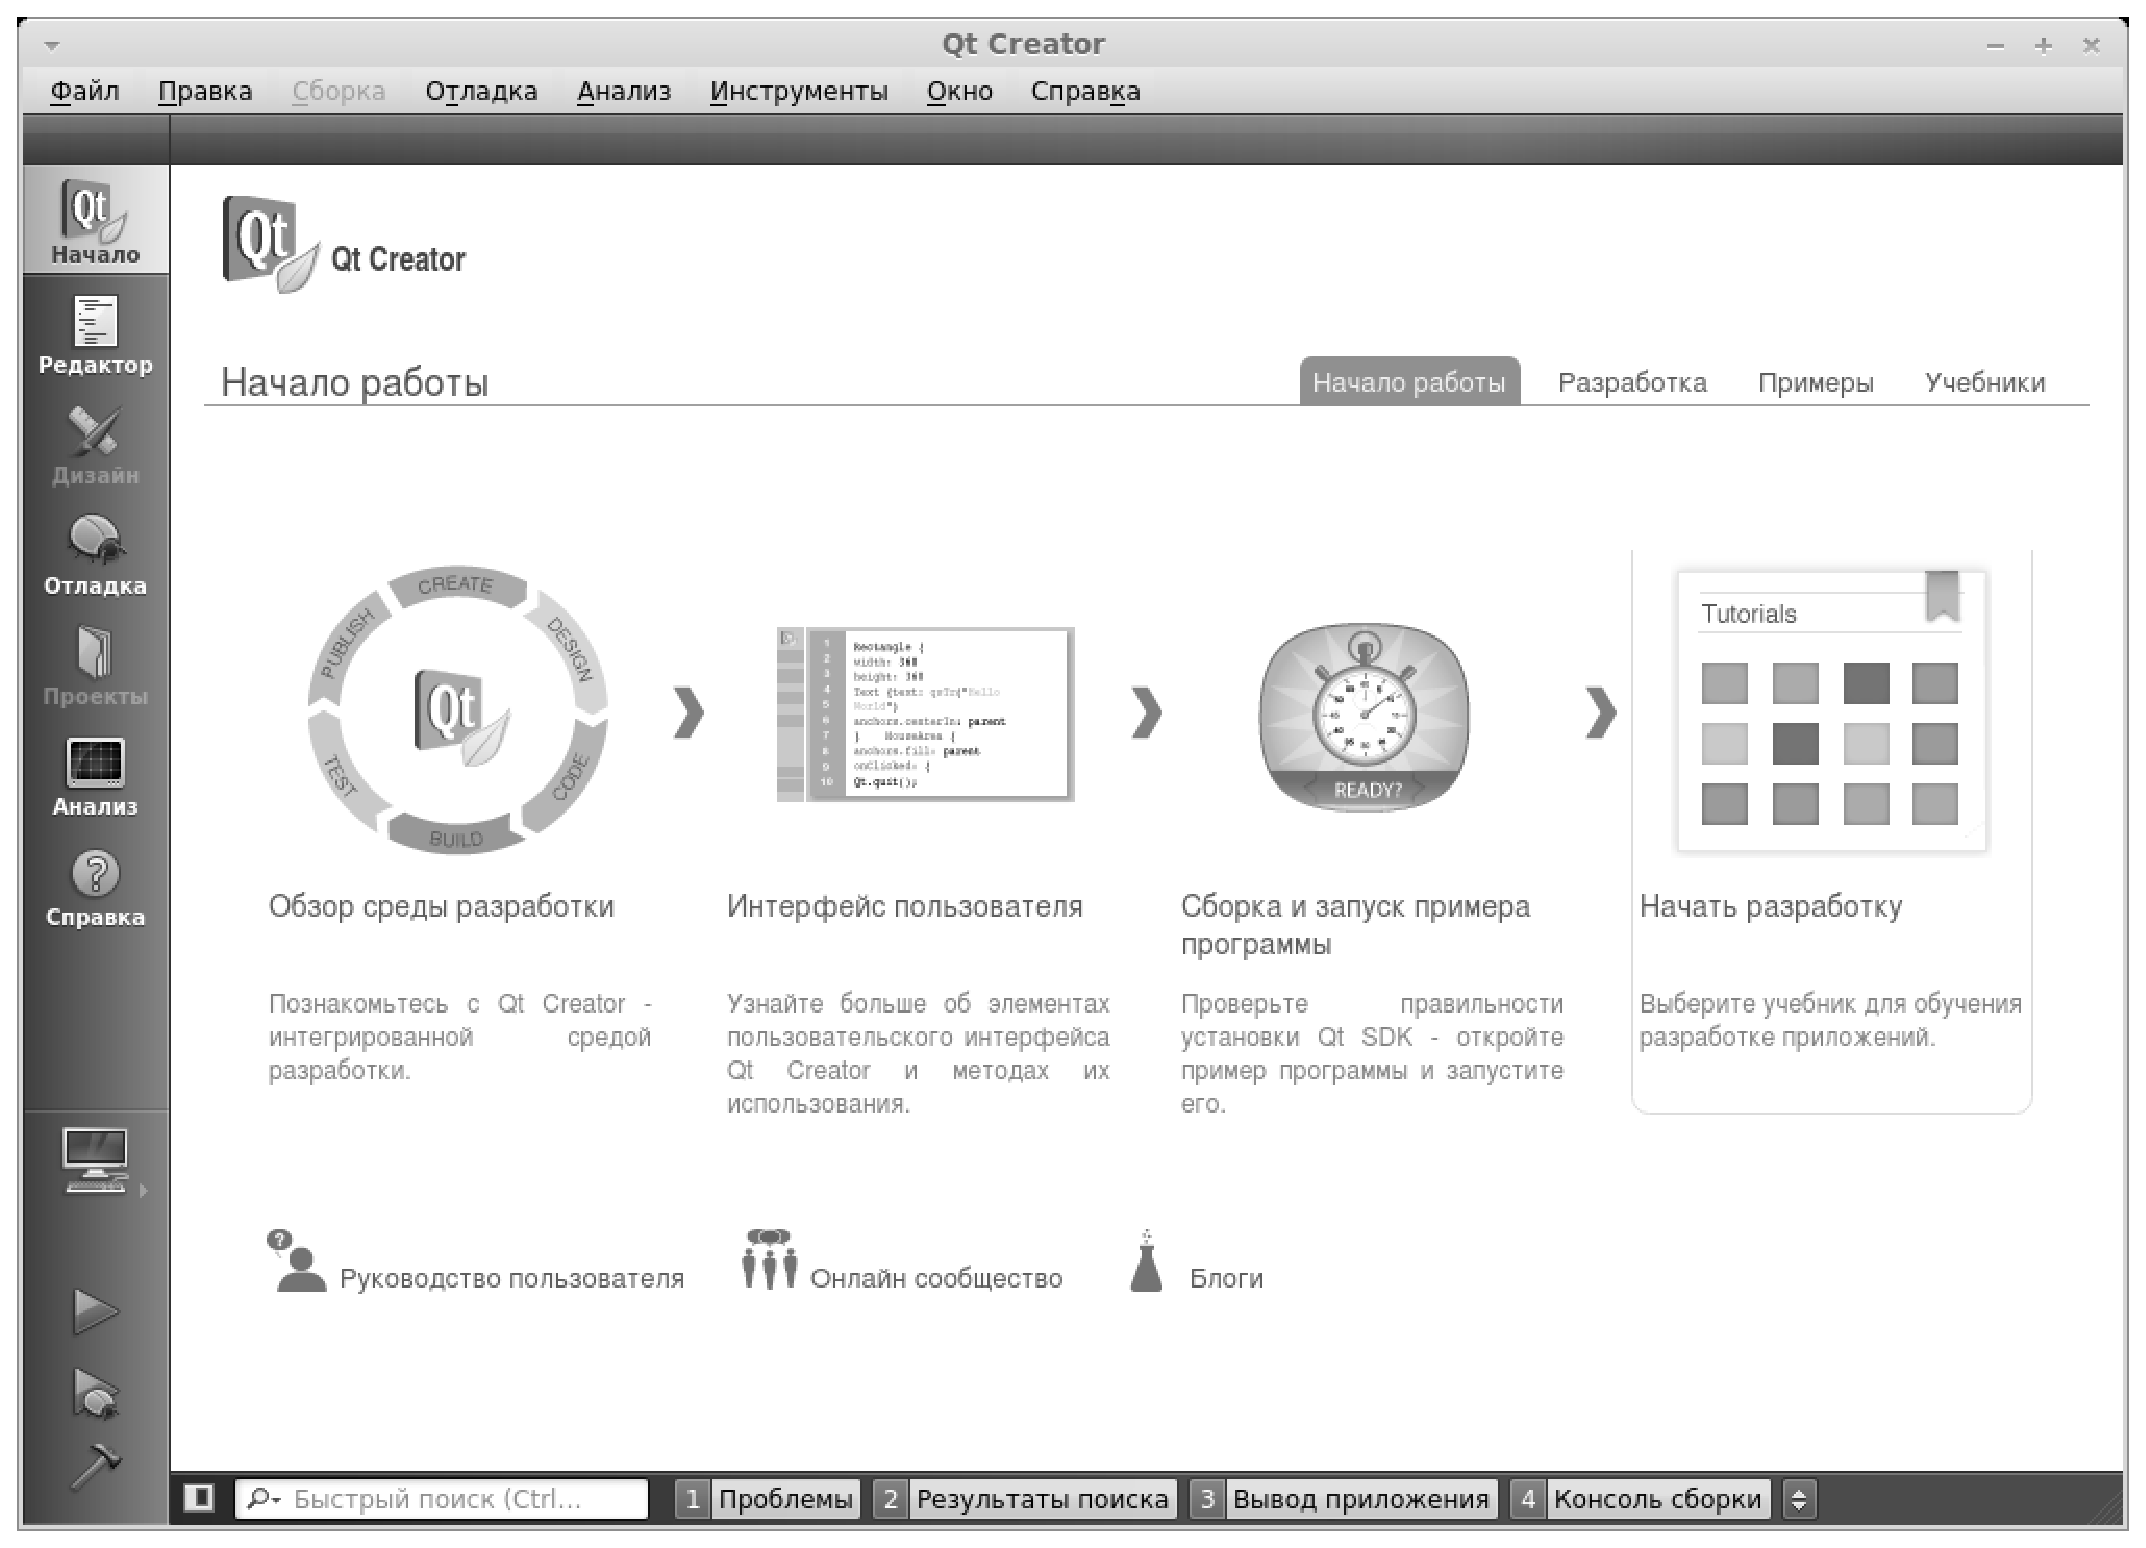
\includegraphics[width=0.8\textwidth]{img/ris_1_1_rus}
\caption{Окно \Sys{Qt Creator}}
\label{ch01:refDrawing0}
\end{center}
\end{figure}
При работе в \Sys{Qt Creator} вы находитесь в одном из режимов:

\begin{enumerate}
\item \Emph{Welcome} (Начало) --- отображает экран приветствия, позволяя быстро загружать недавние сессии или отдельные
проекты. Этот режим можно увидеть при запуске \Sys{Qt Creator} без указания ключей командной строки.
\item \Emph{Edi}t (Редактор) --- позволяет редактировать файлы проекта и исходных кодов. Боковая панель слева
предоставляет различные виды для перемещения между файлами.
\item \Emph{Debug} (Отладка) --- предоставляет различные способы для просмотра состояния программы при отладке;
\item \Emph{Projects} (Проекты) --- используется для настройки сборки, запуска и редактирования кода.
\item \Emph{Analyze} (Анализ) --- в Qt интегрированы современные средства анализа кода разрабатываемого приложения.
\item \Emph{Help} (Справка) --- используется для вывода документации библиотеки Qt и \Sys{Qt Creator}.
\item \Emph{Output} (Вывод) --- используется для вывода подробных сведений о проекте.
\end{enumerate}
Рассмотрим простейшие приёмы работы в среде \Sys{Qt Creator} на примере \index{Консольное приложение!создание}создания
консольного приложения для решения задачи \ref{gl1:prg1}. Для этого можно поступить одним из способов:

\begin{enumerate}
\item В меню \Emph{File} (Файл) выбрать команду \Emph{New File or Project} (Новый файл или проект) (комбинация
клавиш \Emph{Ctrl+N}).
\item Находясь в режиме \Emph{Welcome} (Начало) главного окна QtCreator (рис. \ref{ch01:refDrawing0}) щёлкаем по ссылке
\Emph{Develop} (Разработка) и выбираем команду Create Project (Создать проект).
\end{enumerate}
После это откроется окно, подобное представленному на рис.~\ref{ch01:refDrawing1}. Для создания простейшего консольного
приложения выбираем \Emph{Non-Qt Project} (Проект без использования Qt) --- \Emph{Plain \Sys{C++} Project} (Простой проект
на языке~\Sys{С++}).

Далее выбираем имя проекта и каталог для его размещения (см. рис.~\ref{ch01:refDrawing2})\footnote{Рекомендуем для
каждого (даже самого простого) проекта выбирать отдельный каталог. Даже самый простой проект --- это несколько
взаимосвязанных между собой файлов и каталогов.}. Следующие два этапа создания нашего первого приложения оставляем без
изменения\footnote{О назначении этих этапов будет рассказано в дальнейших разделах книги.}. После чего окно \Sys{IDE Qt
Creator} примет вид, подобное, представленное на рис.~\ref{ch01:refDrawing3}. Заменим текст текста стандартного
приложения, которое выводит текст «Hello, Word», на текст программы решения задачи~\ref{gl1:prg1}.

\begin{figure}[htb]
\begin{center}
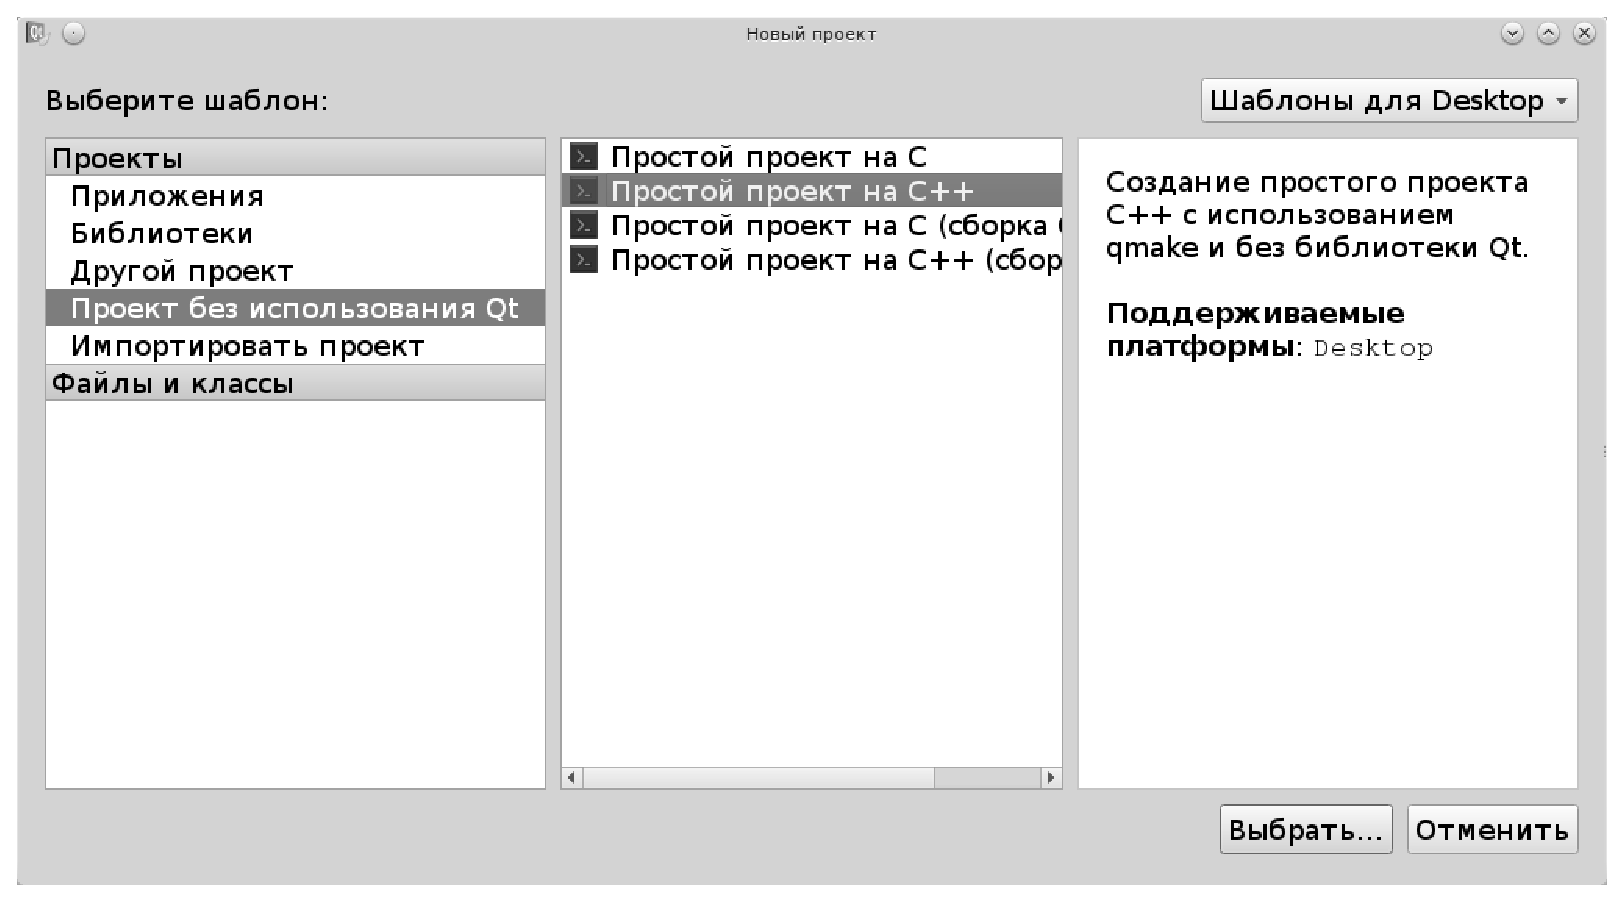
\includegraphics[width=0.8\textwidth]{img/ris_1_2_rus}
\caption{Окно выбора типа приложения в \Sys{Qt Creator}}
\label{ch01:refDrawing1}
\end{center}
\end{figure}

\begin{figure}[htb]
\begin{center}
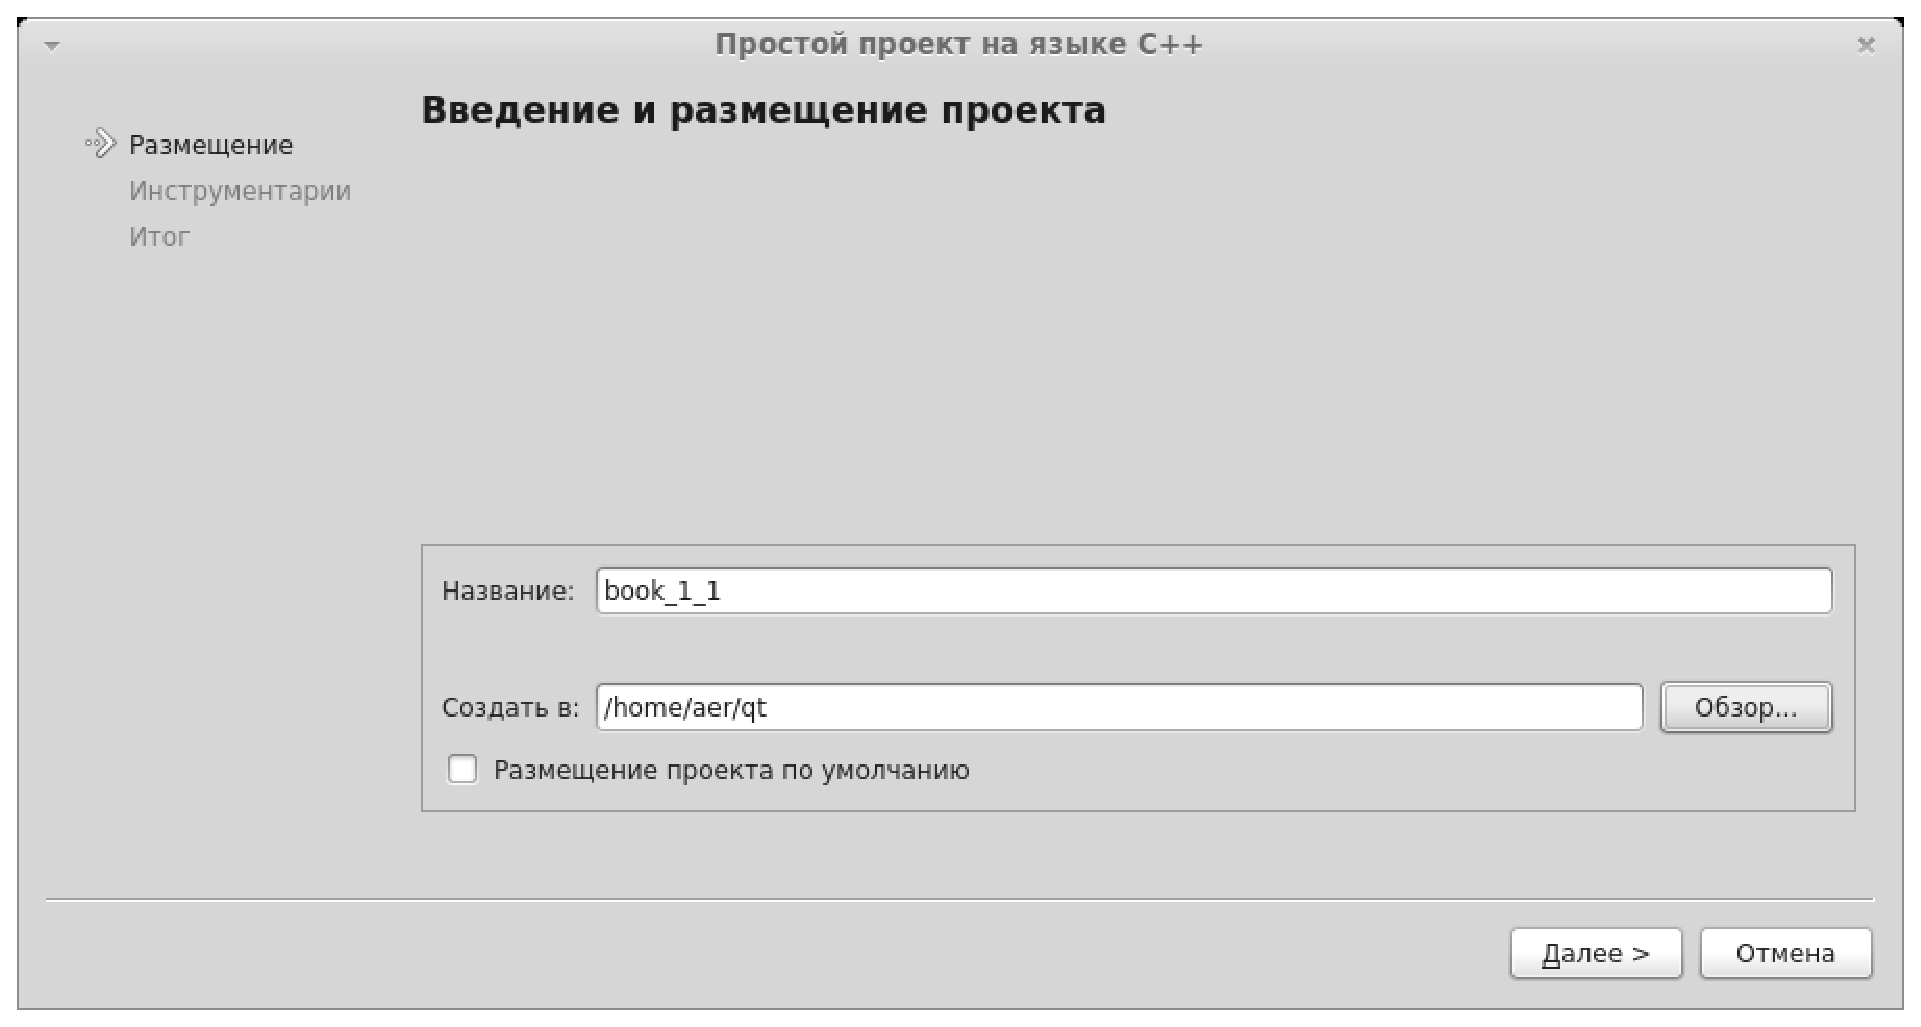
\includegraphics[width=0.8\textwidth]{img/ris_1_3_rus}
\caption{Выбор имени и каталога нового проекта}
\label{ch01:refDrawing2}
\end{center}
\end{figure}

Для сохранения текста программы можно воспользоваться \Emph{Сохранить} или \Emph{Сохранить всё} из меню
\Emph{Файл}. Откомпилировать и \index{Консольное приложение!запуск}запустить программу можно одним из следующих
способов:

\begin{figure}[htb]
\begin{center}
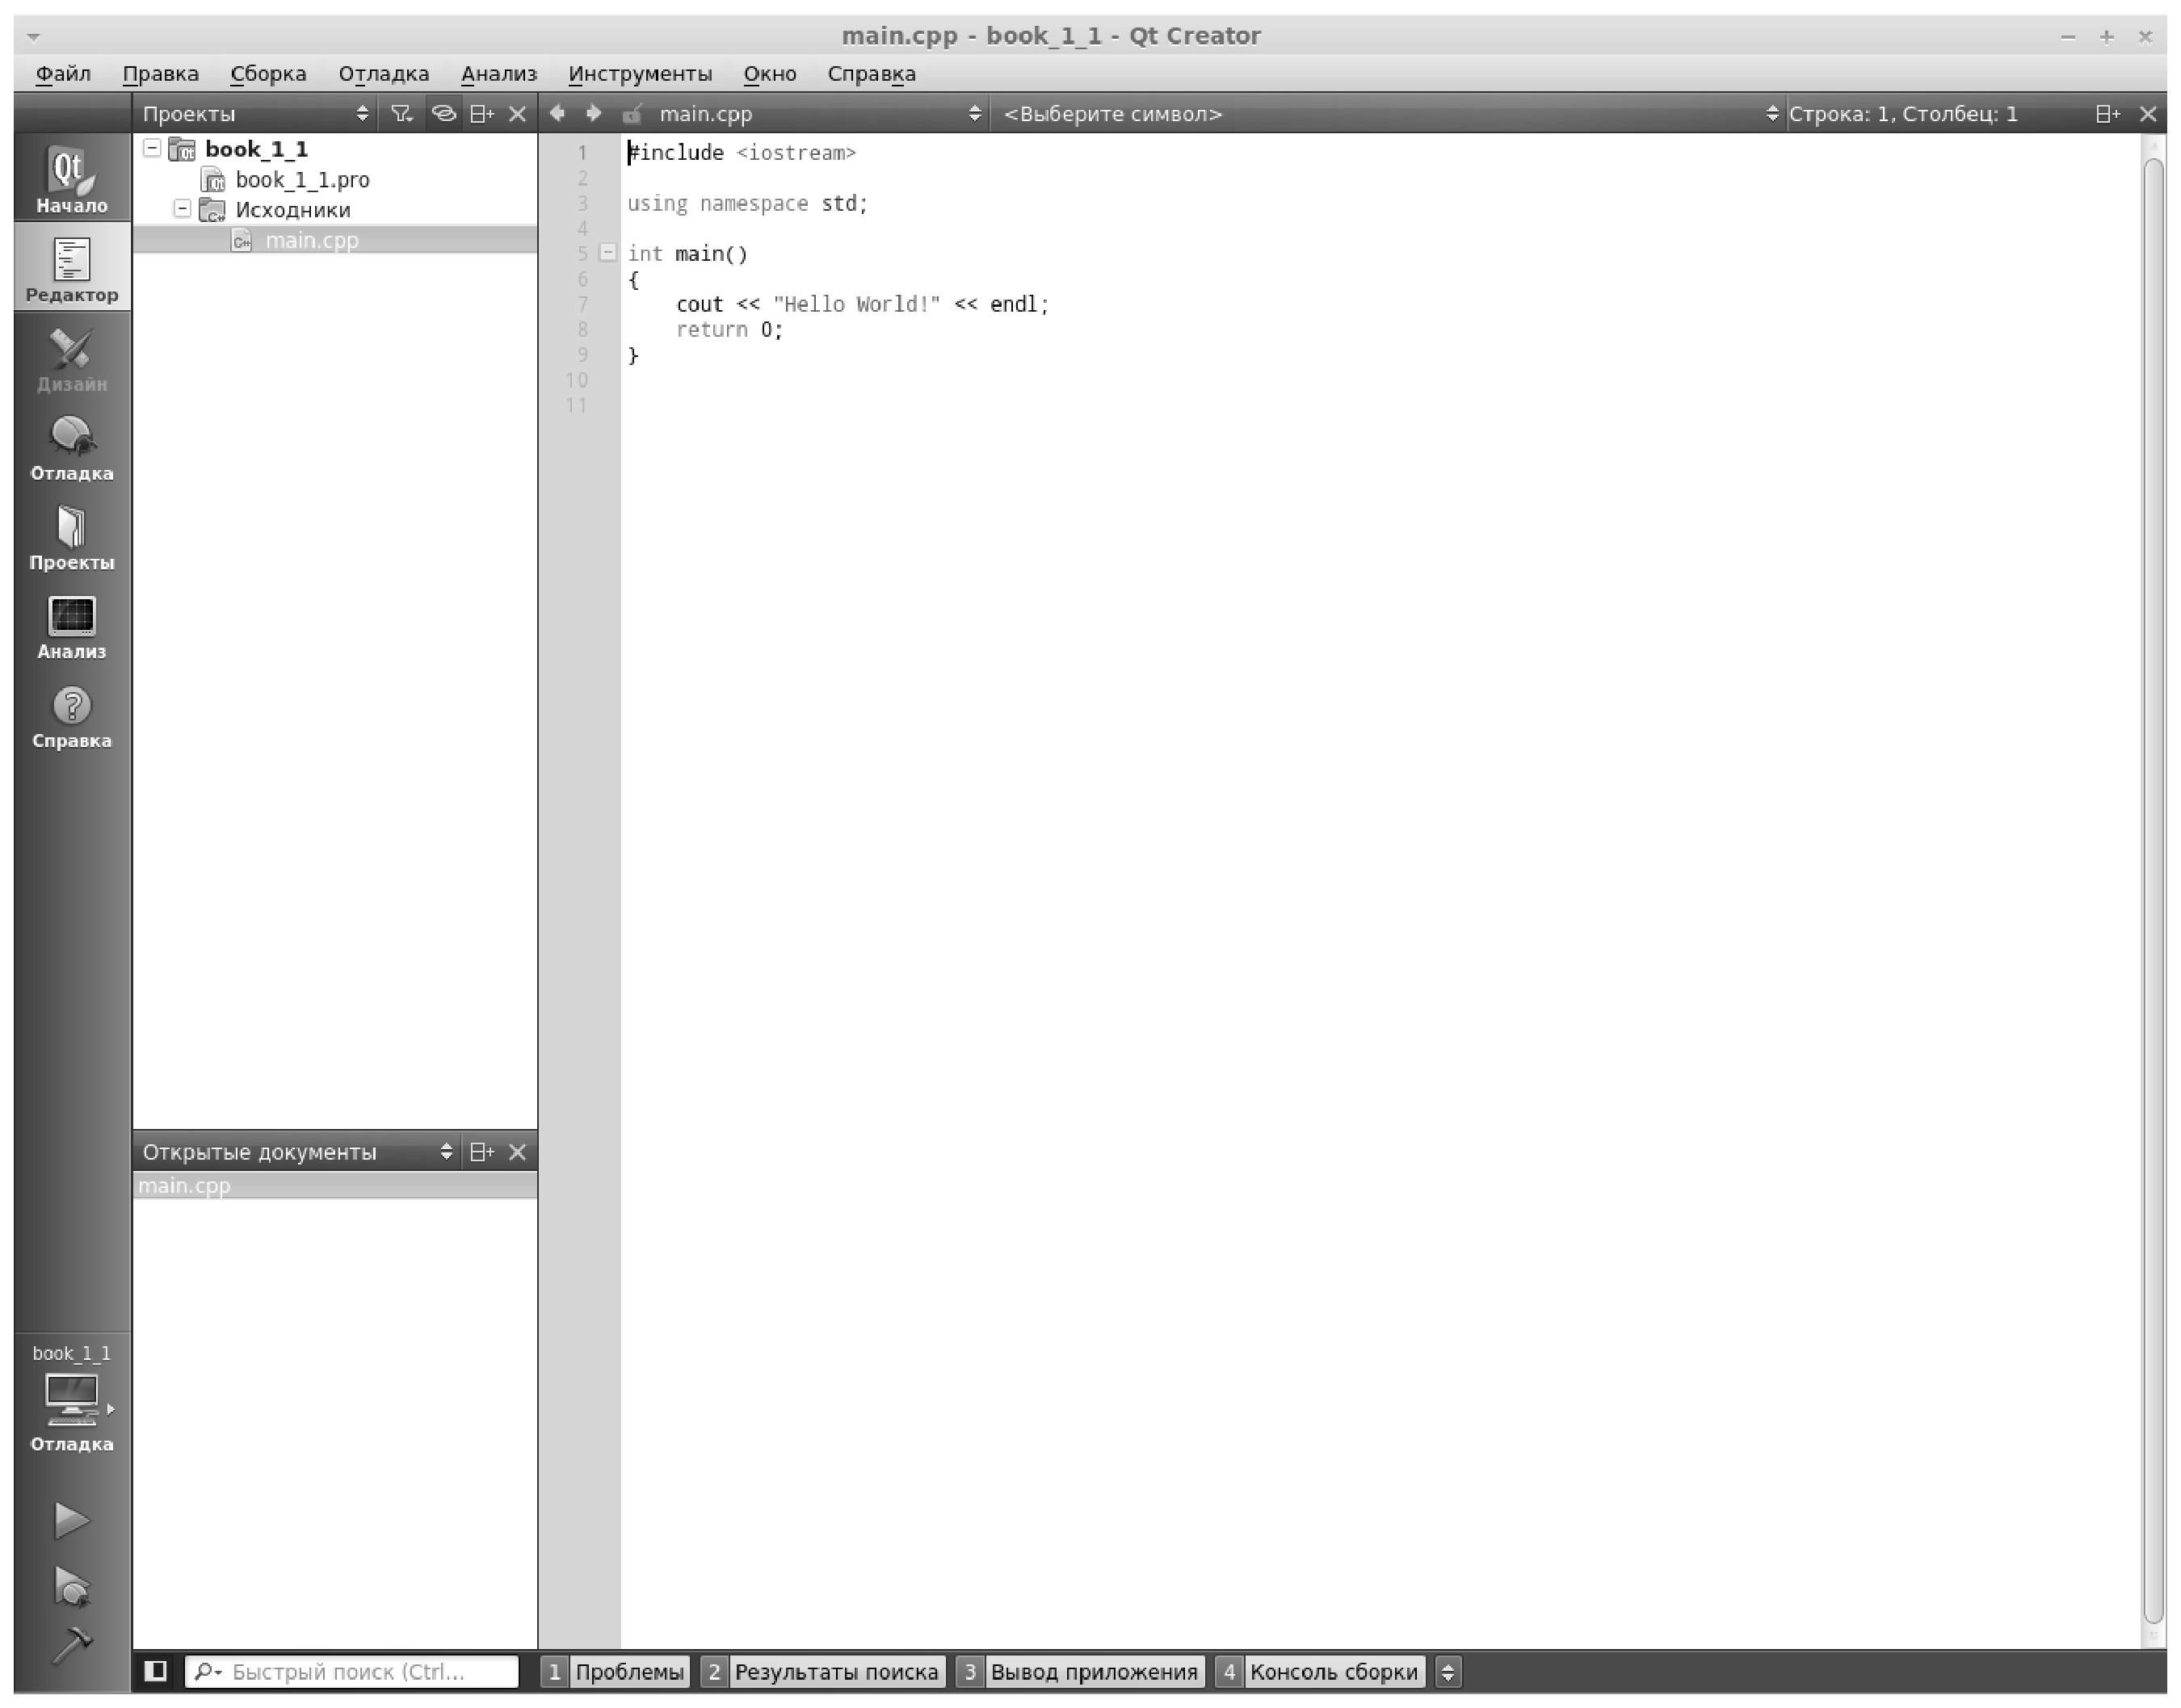
\includegraphics[width=0.8\textwidth]{img/ris_1_4_rus}
\caption{Главное окно создания консольного приложения}
\label{ch01:refDrawing3}
\end{center}
\end{figure}

\begin{enumerate}
\item Пункт меню \Emph{Сборка-Запустить}.
\item Нажать на клавиатуре комбинацию клавиш Ctrk+R.
\item Щёлкнуть по кнопке Запустить (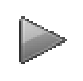
\includegraphics[scale=0.33]{img/rightarrow}).
\end{enumerate}
Окно с результатами работы программы представлено на рис. \ref{ch01:refDrawing4}.
\begin{figure}[htb]
\begin{center}
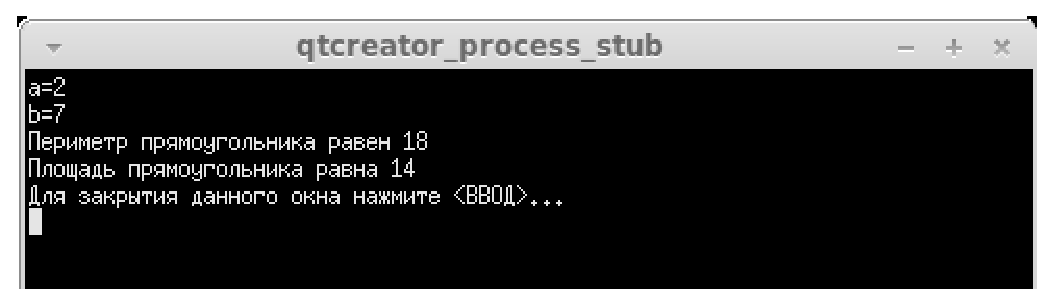
\includegraphics[width=0.8\textwidth]{img/ris_1_5}
\caption{Результаты работы программы решения задачи~\ref{gl1:prg1}}
\label{ch01:refDrawing4}
\end{center}
\end{figure}

Авторы сталкивались с тем, что в некоторых дистрибутивах Ubuntu Linux и Linux Mint после установки \Sys{Qt Creator} не
запускались консольные приложения. Если читатель столкнулся с подобной проблемой, скорее всего надо корректно настроить
терминал, который отвечает за запуск приложений в консоли. Для этого вызываем команду Tools --- Options --- Environment
(см. рис.~\ref{ch01:refDrawing5}). Параметр \Emph{Terminal} (Терминал) должен быть таким же, как показано на рис.
\ref{ch01:refDrawing5}. Проверьте установлен ли в Вашей системе пакет xterm, и при необходимости доставьте его. После
этого не должно быть проблем с запуском консольных приложений.

\begin{figure}[htb]
\begin{center}
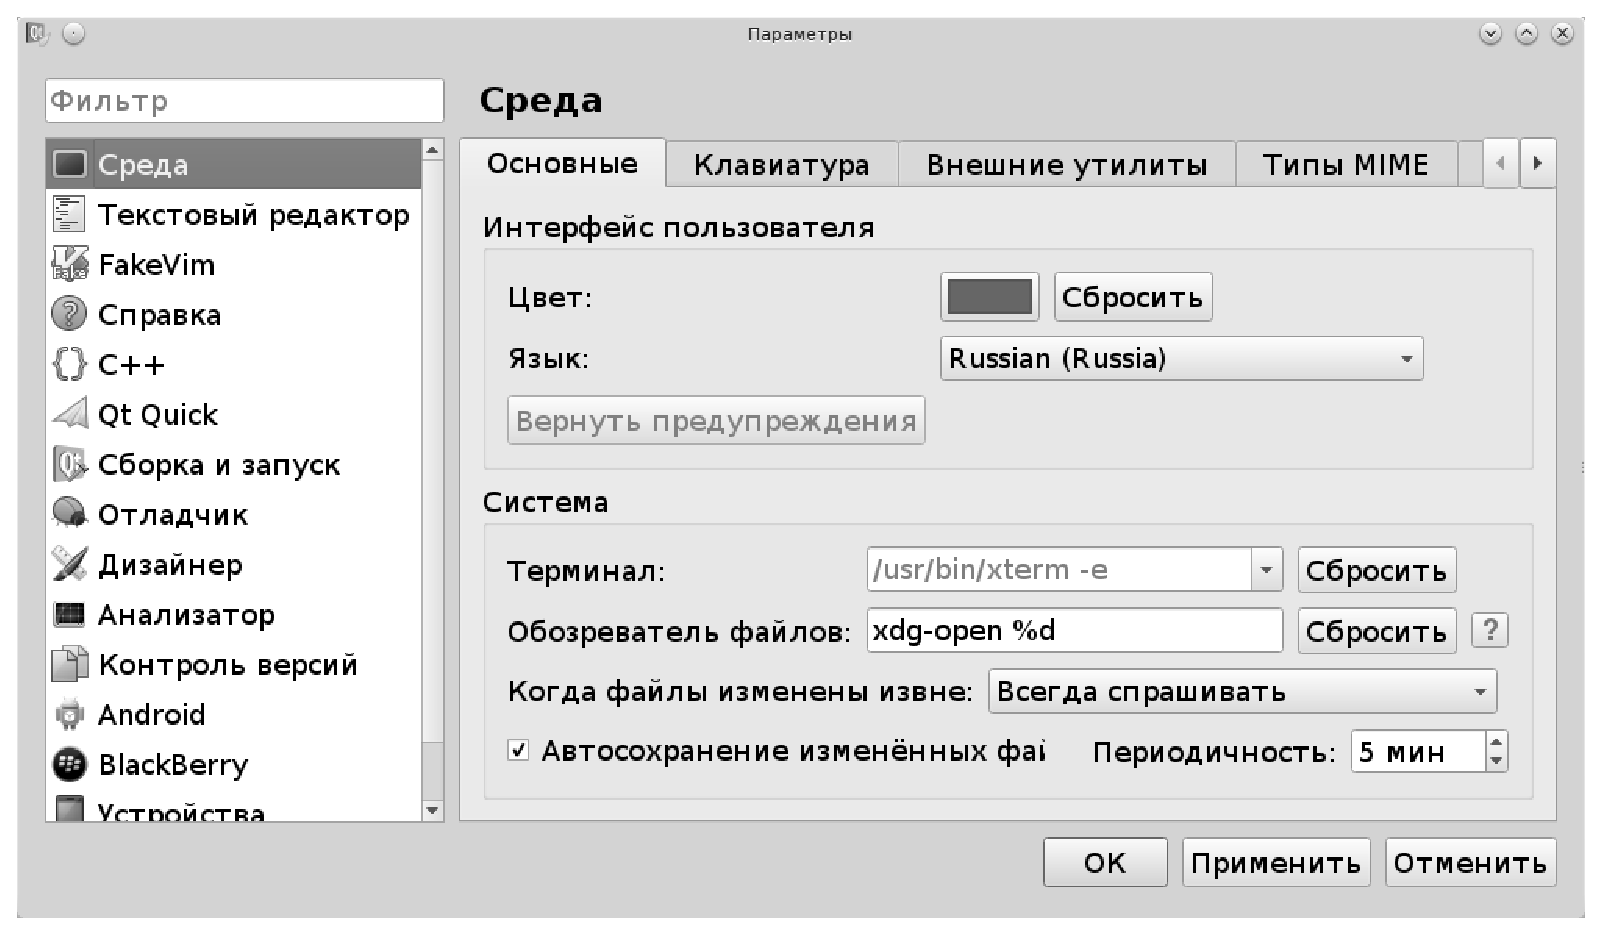
\includegraphics[width=0.8\textwidth]{img/ris_1_6}
\caption{Окно настроек среды \Sys{Qt Creator}}
\label{ch01:refDrawing5}
\end{center}
\end{figure}


Аналогичным образом можно создавать и запускать любое консольное приложение.

Дальнейшее знакомство со средой \Sys{Qt Creator} продолжим, решая следующую задачу.

\prg{Заданы длины трёх сторон треугольника a, b и c (см. рис.~\ref{ch01:refDrawing6}). 
Вычислить площадь и периметр треугольника}{gl1_prg2}

\begin{figure}[htb]
\begin{center}
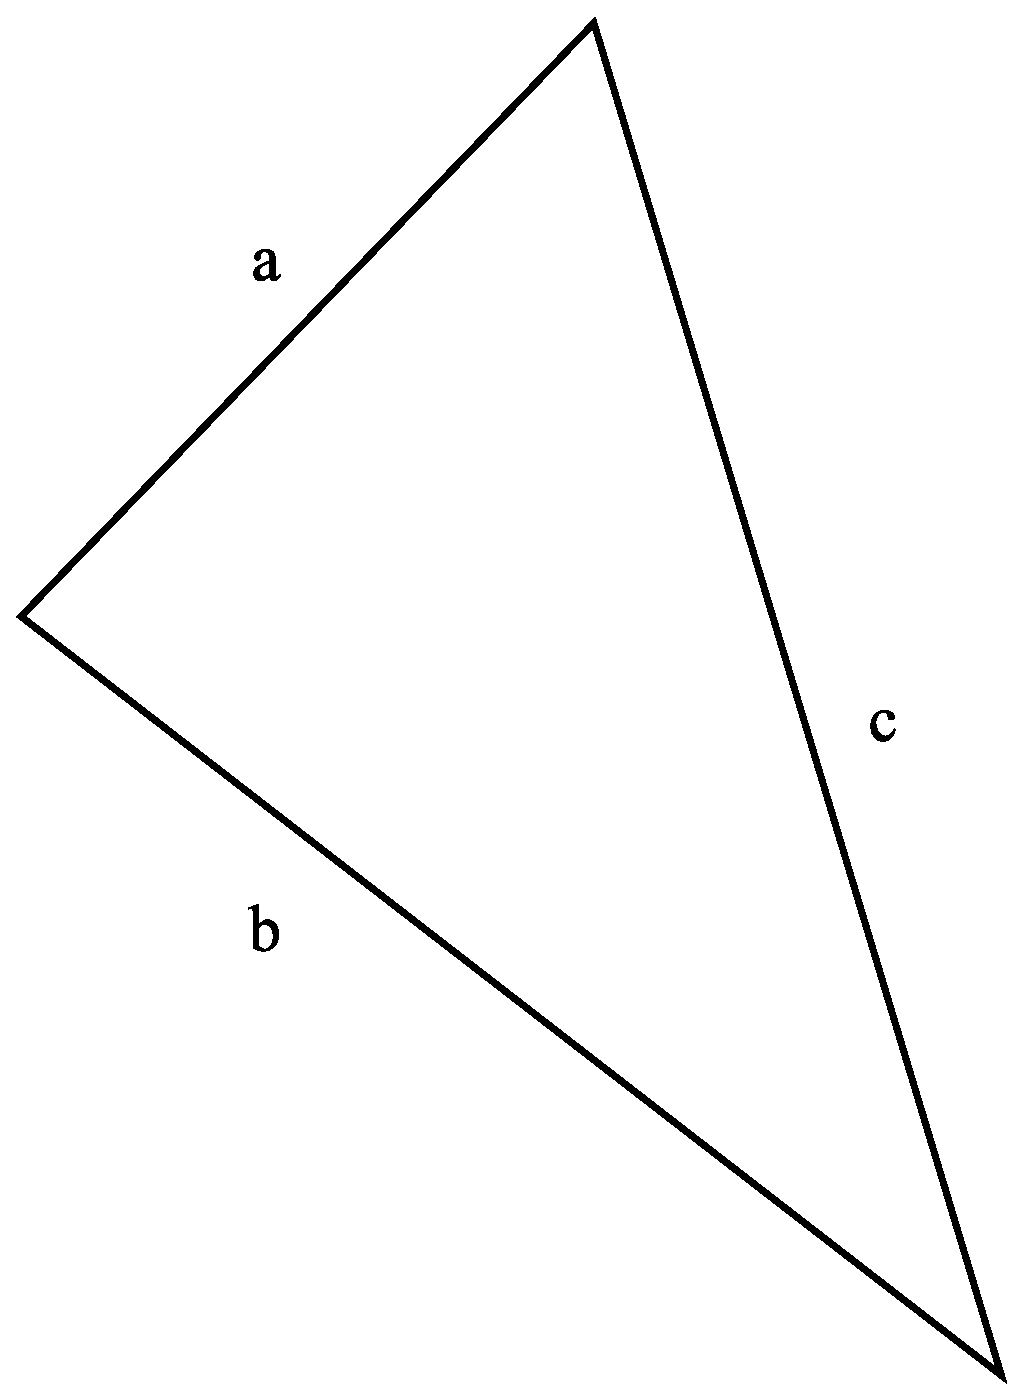
\includegraphics[width=0.3\textwidth]{img/ris_1_7}
\caption{Треугольник}
\label{ch01:refDrawing6}
\end{center}
\end{figure}

Для решения задачи нам понадобится формула вычисления периметра  $p=a+b+c$. Для вычисления площади можно воспользоваться
формулой Герона  $S=\sqrt{\frac{p}{2}\left(\frac{p}{2}-a\right)\left(\frac{p}{2}-b\right)\left(\frac{p}{2}-a\right)}$.

Решение задачи можно разбить на следующие этапы:

\begin{enumerate}
\item  Определение значений a, b и c (ввод величин a, b, c с клавиатуры в память компьютера).
\item  Расчет значений p и s по приведенным выше формулам.
\item Вывод p и s на экран дисплея.
\end{enumerate}
Ниже приведен текст программы. Сразу заметим, что в тексте могут встречаться строки, начинающие с двух наклонных (//),
являющиеся комментариями. \emph{Комментарии}%
%{\textless}!{}-{}-[if supportFields{]}{\textgreater}{\textless}span
%style={}'mso{}-element:field{}-end{}'{\textgreater}{\textless}/span{\textgreater}{\textless}![endif{]}{}-{}-{\textgreater}
%12 Февраль 2013 г. 20:27
~не являются обязательными элементами программы и ничего не сообщают компьютеру, они поясняют человеку, читающему текст
программы, назначение отдельных элементов программы. В книге комментарии будут широко использоваться для пояснения
отдельных участков программы.
\begin{lstlisting}
#include <iostream> 
#include <math.h> 
using namespace std; 
int main() 
{ 
    float a,b,c,s,p; 
    cout<<"`Введите длины сторон треугольника`"<<endl; 
//`Ввод значений длин треугольника` a,b,c.
    cin>>a>>b>>c; 
//`Вычисление периметра треугольника`.
    p=a+b+c; 
//`Вычисление площади треугольника`.
    s=sqrt(p/2*(p/2-a)*(p/2-b)*(p/2-c));
//`Вывод на экран дисплея значений площади и периметра треугольника.` 
    cout<<"`Периметр треугольника равен` "<<p<<", `его площадь равна` "<<s<<endl; 
    return 0; 
}
\end{lstlisting}

Кроме используемой в предыдущей программе библиотеки \Sys{iostream}, в строке 2 подключим библиотеку
\index{Библиотека!math.h}\Sys{math.h}, которая служит для использования математических 
функций языка \Sys{С}(\Sys{С++}). В данной
программе используется функция извлечения квадратного корня --- \index{Функция!sqrt(x)}\emph{sqrt(x)}. Остальные
операторы (ввода, вывода, вычисления значений переменных аналогичны используемым в предыдущей программе.

Таким образом, выше были рассмотрены самые простые программы (линейной структуры), которые предназначены для ввода
исходных данных расчёта по формулам и вывода результатов.

